\documentclass[a4paper,norsk, 10pt]{article}
\usepackage[utf8]{inputenc}
\usepackage{verbatim}
\usepackage{listings}
\usepackage{graphicx}
\usepackage[norsk]{babel}
\usepackage{a4wide}
\usepackage{color}
\usepackage{amsmath}
\usepackage{float}
\usepackage{amssymb}
\usepackage[dvips]{epsfig}
\usepackage[toc,page]{appendix}
\usepackage[T1]{fontenc}
\usepackage{cite} % [2,3,4] --> [2--4]
\usepackage{shadow}
\usepackage{hyperref}
\usepackage{titling}
\usepackage{marvosym }
\usepackage{subcaption}
\usepackage[noabbrev]{cleveref}
\usepackage{cite}


\setlength{\droptitle}{-10em}   % This is your set screw

\setcounter{tocdepth}{2}

\lstset{language=c++}
\lstset{alsolanguage=[90]Fortran}
\lstset{alsolanguage=Python}
\lstset{basicstyle=\small}
\lstset{backgroundcolor=\color{white}}
\lstset{frame=single}
\lstset{stringstyle=\ttfamily}
\lstset{keywordstyle=\color{red}\bfseries}
\lstset{commentstyle=\itshape\color{blue}}
\lstset{showspaces=false}
\lstset{showstringspaces=false}
\lstset{showtabs=false}
\lstset{breaklines}
\title{FYS2140, Oblig 1}
\author{Daniel Heinesen, daniehei}
\begin{document}
\maketitle

\section*{2.4)}

\subsection*{a)}
Den fotoelektriske effektien beskriver fenomenet hvor fotoner slår elektroner ut av atomer, og dermed kan skape en strøm. På slutten av 1800-tallet mente man at lys var bølger som kunne ha kontinuelig energi. Men eksperimenter \ref{fig::fotoele} vise at energien til elektronene ikke var avhengig av intensiteten til lyset, noe man kan forvente fra kontinuelig energi. Høyere intensitet økte strømmen produsert av elektronene, men det viste seg at det var en øvre grense for energien til elektronet, og denne grensen var helt uavhengig av intensiteten til lyset. Når man så på $K_{max}$ som en funksjon av frekvensen til lyset, fant man en klar lineær sammenheng, som sa at energien til et foton kunne skrives som:

$$
E = h\nu
$$

Man kunne da tenke på fotoner som partikler, og ikke lenger som bølger. Det eneste høyere intensitet gjorde var å sende flere av disse partiklene som løsnet flere elektroner, men de hadde ikke mer kinetisk energi.\\

Det var en av de største skrittene mot kvantefysikken.



\begin{figure}[H]
\centering
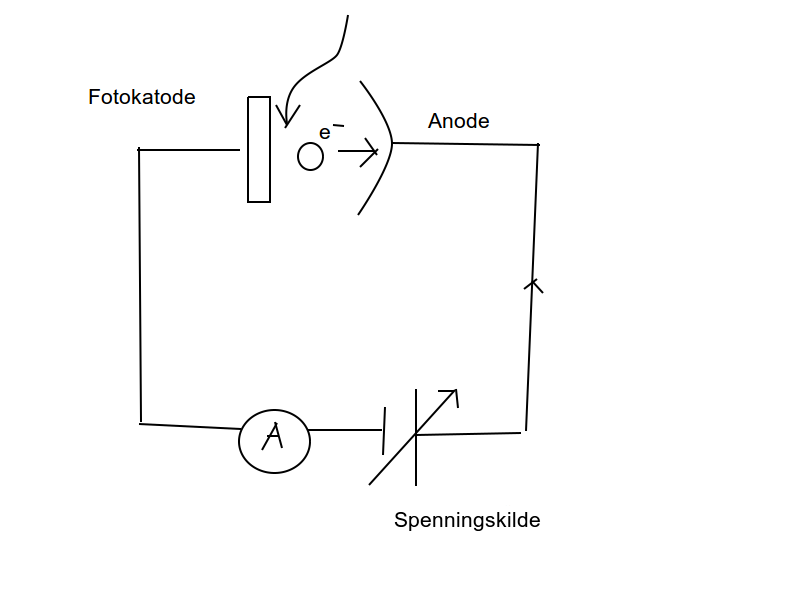
\includegraphics[scale=0.4]{fotoel.png}
\caption{Viser oppsettet til eksperimentet for å vise den fotoelektriske effekten.}\label{fig::fotoele}
\end{figure}

\subsection*{b)}
Grafen viser strømmen som en funksjon av spenning fra spenningskilden. Når spenningen er over 1V vil alle de løsrevede elektonene nå anoden. Så selv om man tilsetter mer spenning, så ikke det øke spenningen siden alle elektronene allerede har nok energi. Senker man spenningen vil ikke lenger alle elektronene ha nok kinetisk energi til å nå anoden, og strømmen vil synke. Selv om spenningen er under null vil noen av elektronene nå anoden. Men ved en $-V_0$ vil plutselig ingen elektronen nå anoden, selv ikke de elektronene som hadde høyest energi. Denne grensen er uavhengig av intensiteten til lyset. Ette viser at elektronene har en høyest mulig energi $K_{max}$ som er uavhengig av intensiteten til lyset.\\

Som nevt over vil ikke $-V_0$ ender seg selv om man dobler intensiteten til lyset. Men etter dette punket vil grafen ligge over grafen for den initielle intensiteten, m.a.o blir det mer strøm i kretsen. Dette er fordi høyere intensitet gir flere fotoner, som igjen river flere elektroner løs. Disse elektronene har ikke noe høyere kinetisk energi, men siden det er flere av dem vil man få høyere strøm.

\subsection*{c)}
Vi vet at for lyset brukt for dette plottet er $\lambda = 2.57 \cdot 10^{-7}$m. Vi vet også at $K_{max} = eV_0 = -0.6$eV. Arbeidsfunksjonen $\omega_0$ er energien som trenges for å rive et elektron vekk fra atomet, og vi kan finne den fra 

$$
K_{max} = h\nu - \omega_0
$$
$$
\omega_0 = h\nu - K_{max}
$$

Setter vi inn de kjente verdiene finner vi at $\omega_0 = 5.42 \mathrm{eV} = 8.7 \cdot 10^{-19}$J

\subsection*{d)}
Med dataen tabell 2 i kompendiumet kan vi finne arbeidsfunksjonen. Vi kan plotte $\nu = \frac{c}{\lambda}$ mot $K_{max} = eV_0$ 

\begin{figure}[H]
\centering
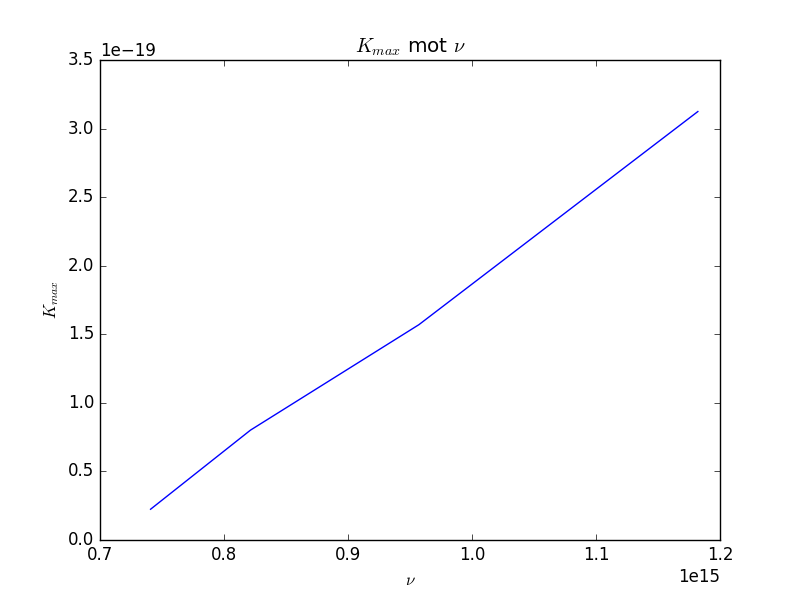
\includegraphics[scale=0.3]{kmaxnu.png}
\caption{Vi kan se at plottet $\nu$ mot $K_{max}$ gir en lineær funksjon.}
\end{figure}

Ved lineær regresjon finner vi at dette følger:

$$
K_{max} = 6.50458\cdot 10^{-34} \nu - 4.58918\cdot 10^{-19}
$$

Det betyr at arbeidsfunksjonen hvor elektronet blir revet løs fra atomet er $\omega_0 = 4.58918\cdot 10^{-19} $J. Vi vet at

$$
K_{max} = h\nu - \omega_0
$$

Som betyr at vi kan finne Planks konstant $h$ ved å se på stigningstallet. Vi finner da at $h = 6.50458\cdot 10^{-34} \mathrm{m}^2 \mathrm{kg}/\mathrm{s}$.

\subsubsection*{e)}\label{subsec::overforingAvAllEnergi}
For å finne ut om et foton kan overføre all energien sin til et elektron, må vi se på bevaring av bevelgelsesmengde og energi. Vi velger et referansepunkt hvor elektronet ikke har noe bevegelsesmengde før sammenstøtet. Fotonet forvinner også etter sammenstøtet og har da verken energi eller bevegelsesmengde. Vi får da at bevegelsesmengdene er:

$$
p_e = p_e
$$
$$
p_{\gamma} = \frac{h}{\lambda}
$$

Og energiene:

$$
E_{e,before} = m_ec^2
$$

$$
E_e = \sqrt{p_e^2c^2 + m_e^2c^4}
$$
$$
E_{\gamma} = \frac{hc}{\lambda}
$$

Bruker vi bevaring og setter inn utrykket for $p_e$ inn i $E_e$ får vi at:

$$
m_ec^2 + \frac{hc}{\lambda} = \sqrt{p_e^2c^2 + m_e^2c^4} = \sqrt{(\frac{h}{\lambda})^2c^2 + m_e^2c^4}
$$

Løser vi opp kvadratroten får vi at

$$
m_e^2c^4 +2\frac{m_ehc^3}{\lambda} + \frac{h^2c^2}{\lambda^2} = \frac{h^2c^2}{\lambda^2} + m_e^2c^4
$$

$$
\Rightarrow 2\frac{m_ehc^3}{\lambda} = 0
$$

Men vi vet at verken $m_e$,$\lambda$ eller $c$ er $0$, og derfor er $2\frac{m_ehc^3}{\lambda} \ne 0$. Vi har derfor en motsigelse, hvilket betyr at fotonet ikke kan gi all energien sin til elektronet.

\section*{2.8)}

\subsection*{a)}

\begin{figure}[H]
\centering
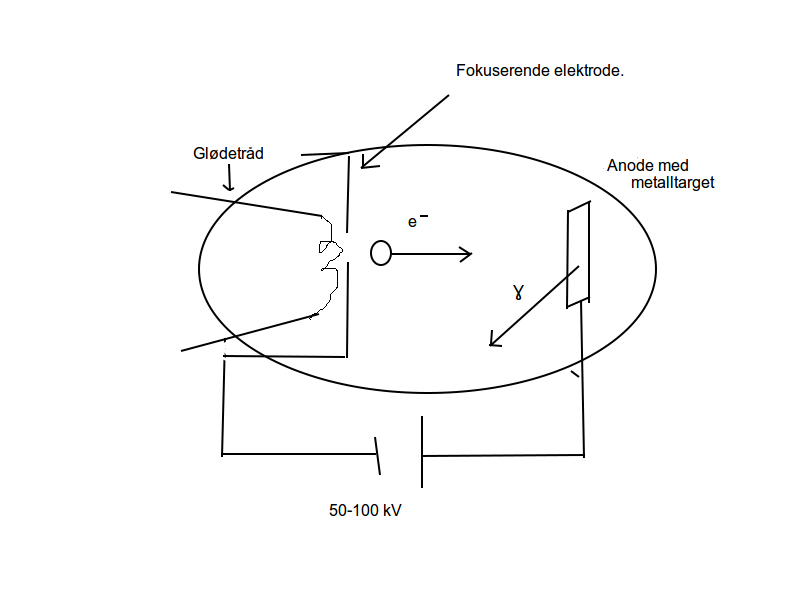
\includegraphics[scale=.4]{rontgen.png}
\caption{Skimatisk tegning av en røtgenrør.}\label{img::rontgenror}
\end{figure}

I figuren over \ref{img::rontgenror} ser vi en enkel tegning av et røtgenrør. Elektroner blir laget av glødetråden og akselereres så mot og igjennom den fokuserende elektroden. Spenningsforskjellen mellom denne elektroden og anoden (rundt 50-100 kV) på forsetter og akselerere elektroden før det tilslutt kræsjer inn i metalltargeten. Inne i metallet vil atomene bremse opp elektronet. Den energien som tapes av elektronet vil gå over i stråling, \textit{Bremsstrahlung}. For systemer som dette vil stråling være i form av røntgenstråling ($\lambda = 0.01 - 10$ nm).

\subsection*{b)}
Fra kompendiumet finner vi at $\lambda_{min}$ ved

$$
\lambda_{min}  = \frac{hc}{eV_R}
$$

Om elektronet har kinetisk energi $K_e = 10000$ eV vil dette gi en minste bølgelengde på:

$$
\lambda_{min} =  \frac{hc}{10000 \mathrm{eV}} = 1.24 \cdot 10^{-10} \mathrm{m}
$$

\subsection*{c)}
Når fotonet treffer krystallen vil en del av lyset reflekteres fra overflaten på krystallen. Noe av lyset vil også igjennom og treffe laget under(eller under der igjen) og reflekteres. Det lyset som reflekteres av laget under vil ha en lengre vei å gå enn det lyset som ble reflektert av overflaten. Dette vil føre til en faseforskyvning. Om avstanden lyset må reise mellom lagene ikke er $n\lambda$ vil fasene til lyset fra de forskjellige lagene ikke være like, og man får destruktiv interferens. Er denne avstanden derimot $n\lambda$ vil fasene være like og lysstrålen vil forsette med samme stryrke men nå i en annen vinkel(refleksjonen). Formelen som beskriver dette (når man får en refleksjon) er:

$$
n\lambda = 2d\sin(\theta)
$$

Vi vet at $\lambda = 1$ nm, $\theta = 45^{\circ}$, og vi er bare interessert i det øverste laget, så vi sier at $n = 1$

$$
d = \frac{\lambda}{2\sin(\theta)} = 0.71 nm
$$

\section*{d)}
Vi ønsker å finne minst mulig fotonenergi $E_{\nu}$ for å få pardannelse. Et elektronpar har minst energi når det står i ro. Den har da ingen bevegelsesmengde, $p_e = 0$. For å finne energien setter vi opp energibevaring. Energien til fotonet $E_{\nu}$, må være like energien til elektronparret etter dannelsen. Vi antar også at fotonet blir borte etter dannelsen. Vi har da at

$$
E_{\nu} = 2\sqrt{p_c^2c^2 + m_e^2c^4}
$$

Men vi vet at elektronet ikke har noe bevegelsesmengde, så vi sitter da igjen med:

$$
E_{\nu} = 2m_ec^2
$$

Med andre ord hvileenergien til de 2 elektronene. Vi har et problem, og det er at selv om energi er bevart, så er ikke bevegelses mengde det. Fotonet hadde trossalt bevegelsesmengde før dannelsen, men det er borte etter, og elektronene står stille. En slik prosess kan derfor bare skje nær en atomkjerne, da det er denne som tar over all bevegelsesmengden til fotonet. Om dette ikke er tilfellet vil ikke denne prosessen være mulig(som sett i oppgave 2.8d \ref{subsec::overforingAvAllEnergi}). Kjernen må også ta over litt av energien til fotonet med bevegelsesmengden. Men vi ønsker her en ideel situasjon, så vi antar at den ikke får noe av energien.

\section*{2.9)}

\subsection*{a)}
Interaksjonen mellom fotonet og elektronet kan sees i figuren under\ref{fig::photonElectronCollision}.

\begin{figure}[H]
\centering
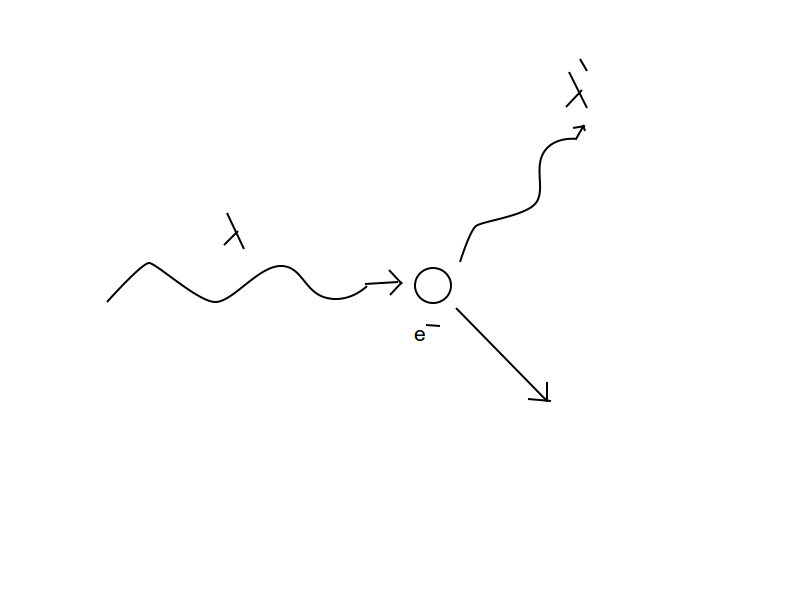
\includegraphics[scale=.3]{comptonLambda.png}
\caption{Figuren viser kollisjonen mellom et foton og et elektron.}\label{fig::photonElectronCollision}
\end{figure}

I en slik kollisjon må både energy og bevegelsesmengde må være bevart. Energiene er gitt som

$$
E_{\gamma} = \frac{hc}{\lambda}
$$
$$
E_e = \sqrt{p_2^2c^2 + m_e^2c^4}
$$

Før kollisjonen står elektronet stille nær kjernen og har bare hvileenergi. Etter har det både en energi og bevegelsesmengde. Før kollisjonen har fotonet bølgelengde $\lambda$ og etter kollisjonen har det $\lambda'$.

Vi skal anta senere at bevegelsesmengden til fotonet er gitt ved

$$
p_{\gamma} = \frac{h}{\lambda}
$$

Men inntil videre skal vi la den stå som ukjent. Før kollisjonen har elektronen ingen bevegelsesmengde, og etter kollisjonen har den en ukjent bevegelsesmengde. Vi kan regne ut denne bevegelesmengden ved å se på bevaring av energien:

$$
m_ec^2 + \frac{hc}{\lambda} = \sqrt{p_2^2c^2 + m_e^2c^4} + \frac{hc}{\lambda'}
$$

Hvilket gir at:

\begin{equation}
p_e^2c^2 = \big(m_ec^2 + \frac{hc}{\Delta \lambda} \big)^2 - (m_ec^2)^2
\end{equation}\label{eq::p2c2}

Hvor $\Delta \lambda = \lambda - \lambda'$.\\

Vi bruker så bevaring av bevegelsesmengde:

$$
\vec{p_{\gamma}} = \vec{p_e} + \vec{p_{\gamma'}} \Leftrightarrow \vec{p_{e}} = \vec{p_{\gamma}} - \vec{p_{\gamma'}}
$$

Hvor $\vec{p_{\gamma'}}$ er bevegelsesmengden til fotonet etter kollisjonen. Vi finner så at:

$$
(p_e)^2 = \vec{p_e} \cdot \vec{p_e} = p_{\gamma'}^2 + p_{\gamma}^2 - 2p_{\gamma}p_{\gamma'}\cos(\theta)
$$

Vi kan nå bruke antagelsen om bevegelsesmengden til fotonet, og i tillegg ganger vi begge siden med $c^2$

\begin{equation}
(p_ec)^2 = \left(\frac{hc}{\lambda}\right)^2 + \left(\frac{hc}{\lambda'}\right)^2 - 2\left(\frac{hc}{\lambda \lambda'}\right)\cos(\theta)
\end{equation}\label{eq::p2c22}

Vi har nå 2 uttykk vi kan sette like hverandre:

$$
\left(\frac{hc}{\lambda}\right)^2 + \left(\frac{hc}{\lambda'}\right)^2 - 2\left(\frac{hc}{\lambda \lambda'}\right)\cos(\theta) = \big(m_ec^2 + \frac{hc}{\Delta \lambda} \big)^2 - (m_ec^2)^2
$$

Å løse dette for $\Delta \lambda$ er en ren algebraisk oppgave, og for mye å skrive i Latex. Men resultatet man får er Comptons formel:

\begin{equation}
\Delta \lambda = \frac{h}{m_ec}(1-\cos(\theta))
\end{equation}\label{eq::compton}


\subsection*{b)}

Etter en kollisjon må fotonet ha gitt noe av sin energi til elektronet. Energien til fotonet er gitt ved $E = \frac{hc}{\lambda}$. Siden både $h$ og $c$ er konstanter, så må en lavere energi bety en høyere bølgelengde $\lambda$.\\

Vi kan også se det fra Comptorn formelen \ref{eq::compton}. Siden $\cos\theta$ er mindre enn 1, blir $\Delta \lambda > 0$, hvilket betyr at $\lambda < \lambda'$.

\subsection*{c)}
Før kollisjonen har fotonet bevegelsesmengde $p_{\gamma} = \frac{h}{\lambda}$ og elektronet $p_e = - p_{\gamma}$. Etter kollosjonen har de $p_{\gamma}' = \frac{h}{\lambda'}$ og $p_e'$. Bruker vi bevaring av bevegelsesmengde finner vi at:

$$
p_{\gamma} + p_e = p_{\gamma} + (-p_{\gamma}) = 0 = p_e' + p_{\gamma}'
$$

$$
\Rightarrow p_e' = - p_{\gamma}' = -\frac{h}{\lambda'}
$$

Vi bruker så dette utrykket i energibevaring:

$$
E_e + E_{\gamma} = E_e' + E_{\gamma}'
$$
$$
\sqrt{p_e^2c^2 + m_e^2c^4} + \frac{hc}{\lambda} = \sqrt{p_e'^2c^2 + m_e^2c^4} + \frac{hc}{\lambda'}
$$

$$
\sqrt{\frac{h^2c^2}{\lambda^2} + m_e^2c^4} + \frac{hc}{\lambda} = \sqrt{\frac{h^2c^2}{\lambda'^2} + m_e^2c^4} + \frac{hc}{\lambda'}
$$

For at dette skal stemme må $\lambda = \lambda'$. M.a.o. er $\Delta \lambda = 0$

\subsection*{d)}
Se oppgave 2.4d \ref{subsec::overforingAvAllEnergi}


\section*{3.2}
\subsection*{a)}
For å finne spinnet til H-systemet må vi først se på massesenteret til systemet. Det er definert som:

$$
\vec{R} = \frac{m_e}{M}\vec{r_e} + \frac{m_p}{M}\vec{r_p}
$$

Hvor $\vec{r_p}$ og $m_p$ er posisjonen og massen til protonet, $\vec{r_e}$ og $m_e$ er det tilsvarende for elektronet, og $M = m_e + m_p$. Siden vi ikke har noen ekterne krefter kan vi velge at massesenteret er i origo, så

$$
 \frac{m_e}{M}\vec{r_e} + \frac{m_p}{M}\vec{r_p} = 0
$$

Avstanden mellom protonet og elektronet er gitt som

$$
\vec{r} = \vec{r_e} - \vec{r_p}
$$

Vi kan skrive om posisjonen til elektronet og sette det inn i formelen over:

$$
\vec{r} = -\frac{m_p}{m_e}\vec{r_p} - \vec{r_p} = .\frac{m_p + m_e}{m_e}\vec{r_p}
$$ 

Vi skriver om, tar lengden av vektorene og setter at $\mu = \frac{m_em_p}{m_e+m_p}$:

\begin{equation}
r_pm_p = -\mu r
\end{equation}\label{eq::rpmp}

og tilsvarende for elektronet:
\begin{equation}
r_em_e = \mu r
\end{equation}\label{eq::reme}

Vi kan nå bruke formelen for det totale utrykket:

$$
L = \sum_i r_ip_i = r_em_e\frac{dr_e}{t} + r_pm_p\frac{dr_p}{dt}
$$
Bruker vi \ref{eq::rpmp} og \ref{eq::reme} får vi at:

$$
L = r_e\mu \frac{dr}{dt} - r_p \mu \frac{dr}{dt} = (r_e -  r_p)\mu v
$$

Bruker vi nå at $r_e - r_p = r$ og at $v = r\omega$ får vi at

$$
L = r^2 \mu \omega
$$

\subsection*{b)}
Bohr brukte mekanisk likevekt og kvantisering av spin til å finne energien til hydrogenatomet. Vi ønsker å bruke det nye uttrykket for spin for å finne en mer nøyaktig formel for energien. Kvantiseringen av spin sier at:

$$
L = r^2\mu \omega = r\mu v = n\hbar
$$

Som gir os at

\begin{equation}
v^2 = \left(\frac{n\hbar}{r\mu}\right)^2
\end{equation}\label{eq::v2}

Så trenger vi energien for et elektron i bane rundt et proton. Det er gitt ved:

\begin{equation}
E = -\frac{ke^2}{r} + \frac{1}{2}\mu v^2 = -\frac{ke^2}{r} + \frac{ke^2}{2r} = -\frac{ke^2}{2r}
\end{equation}\label{eq::E}

Vi bruker så mekanisk likevekt som sier at:

\begin{equation}
\frac{ke^2}{2r} = \frac{1}{2}\mu v^2
\end{equation}\label{likevekt}

Bytter vi ut $v^2$ med \ref{eq::v2} får vi at:

$$
\frac{ke^2}{2r} = \frac{1}{2}\mu \left(\frac{n\hbar}{r\mu}\right)^2
$$
\begin{equation}
r(n) = \frac{\hbar^2}{\mu ke^2}n^2
\end{equation}\label{r}

Setter vi dette inn i uttrykket for energien \ref{eq::E} ender vi med at:

$$
E = -\frac{\mu e^4k^2}{2\hbar e^2}\frac{1}{n^2}
$$

Bohr anta også at energien elektronene strålte ut i form av fotoner når de gikk mellom orbitaler var gitt ved:

$$
h\nu = E_i - E_f
$$

Vi setter inn utrykket for energi og finner at:

$$
h\nu = \frac{\mu e^4k^2}{2\hbar^2}\left(\frac{1}{n_f^2}-\frac{1}{n_i^2}\right)
$$

Siden $\nu = \frac{c}{\lambda}$ ender vi opp med den modifiserte formelen til Bohr:

\begin{equation}
\frac{1}{\lambda} = \frac{\mu e^4k^2}{2\hbar^2hc}\left(\frac{1}{n_f^2}-\frac{1}{n_i^2}\right)
\end{equation}\label{eq::enoverlambda}

Vi ser at den eneste forskjellen er at vi har $\mu$ istedenfor $m_e$

\subsection*{c)}
I følge Bohrs formel er bølgelengden fra $n_i = 3$ til $n_f = 2$ i Balmer-serien 656.11 nm. I den nye formelen blir det:

$$
\frac{\mu e^4k^2}{2\hbar^2hc}\left(\frac{1}{2^2}-\frac{1}{3^2}\right) = \frac{1}{656.47 nm}
$$

Vi har altså med den nye formelen 656.47 nm, alså en forskjell på 0.36 nm, hvilket er en veldig liten forskjell.

\subsection*{d)}
Vi vet nå at $H_{\alpha} = 656.029$ nm for deuterium. For å finne massen på kjernen løser vi \ref{eq::enoverlambda} for $\mu$

$$
\mu = \frac{1}{\lambda}\left[\frac{ e^4k^2}{2\hbar^2hc}\left(\frac{1}{n_f^2}-\frac{1}{n_i^2}\right)\right]^{-1}
$$

Vi får da at $\mu = 4.723 \cdot 10^{-6} kg$. Vi vet at $\mu = \frac{m_pm_e}{m_p + m_e}$. Vi løser dette for $m_p$, som her tilsvarer massen må kjernen:

$$
m_p = \frac{m_e\mu}{m_e-\mu} 
$$

Jeg har prøvd og prøvd å regne dette ut, men tallene er under maskinpresisjon, så den metoden jeg har prøvd å finne det på virker ikke til å fungere...


\end{document}


